\begin{center} \LARGE \bf Folha de Aprovação \end{center}


\begin{enumerate}
    \item Estas instruções \textbf{não} devem ser entregues aos avaliadores do trabalho nas ocasiões dos TCCs 1 e 2. Portanto, comente a linha que importa este arquivo;
    \item Após a defesa do TCC2, efetue as correções indicadas pela banca;
    \item Valide a versão final do trabalho com seu/sua orientador(a). Ele/Ela irá entregar uma carta de anuência ao coordenador da disciplina de TCC2 indicando estar de acordo com a versão final produzida;
    \item O responsável pela disciplina de TCC2 irá lhe entregar digitalmente um documento PDF com as assinaturas e aprovação dos integrantes da banca;
    \item O referido arquivo deve ser adicionado na pasta source com o nome \texttt{assinaturas.pdf};
    \item Todo o conteúdo deste arquivo deve ser retirado e substituído pelo seguinte comando:

   \begin{verbatim}
       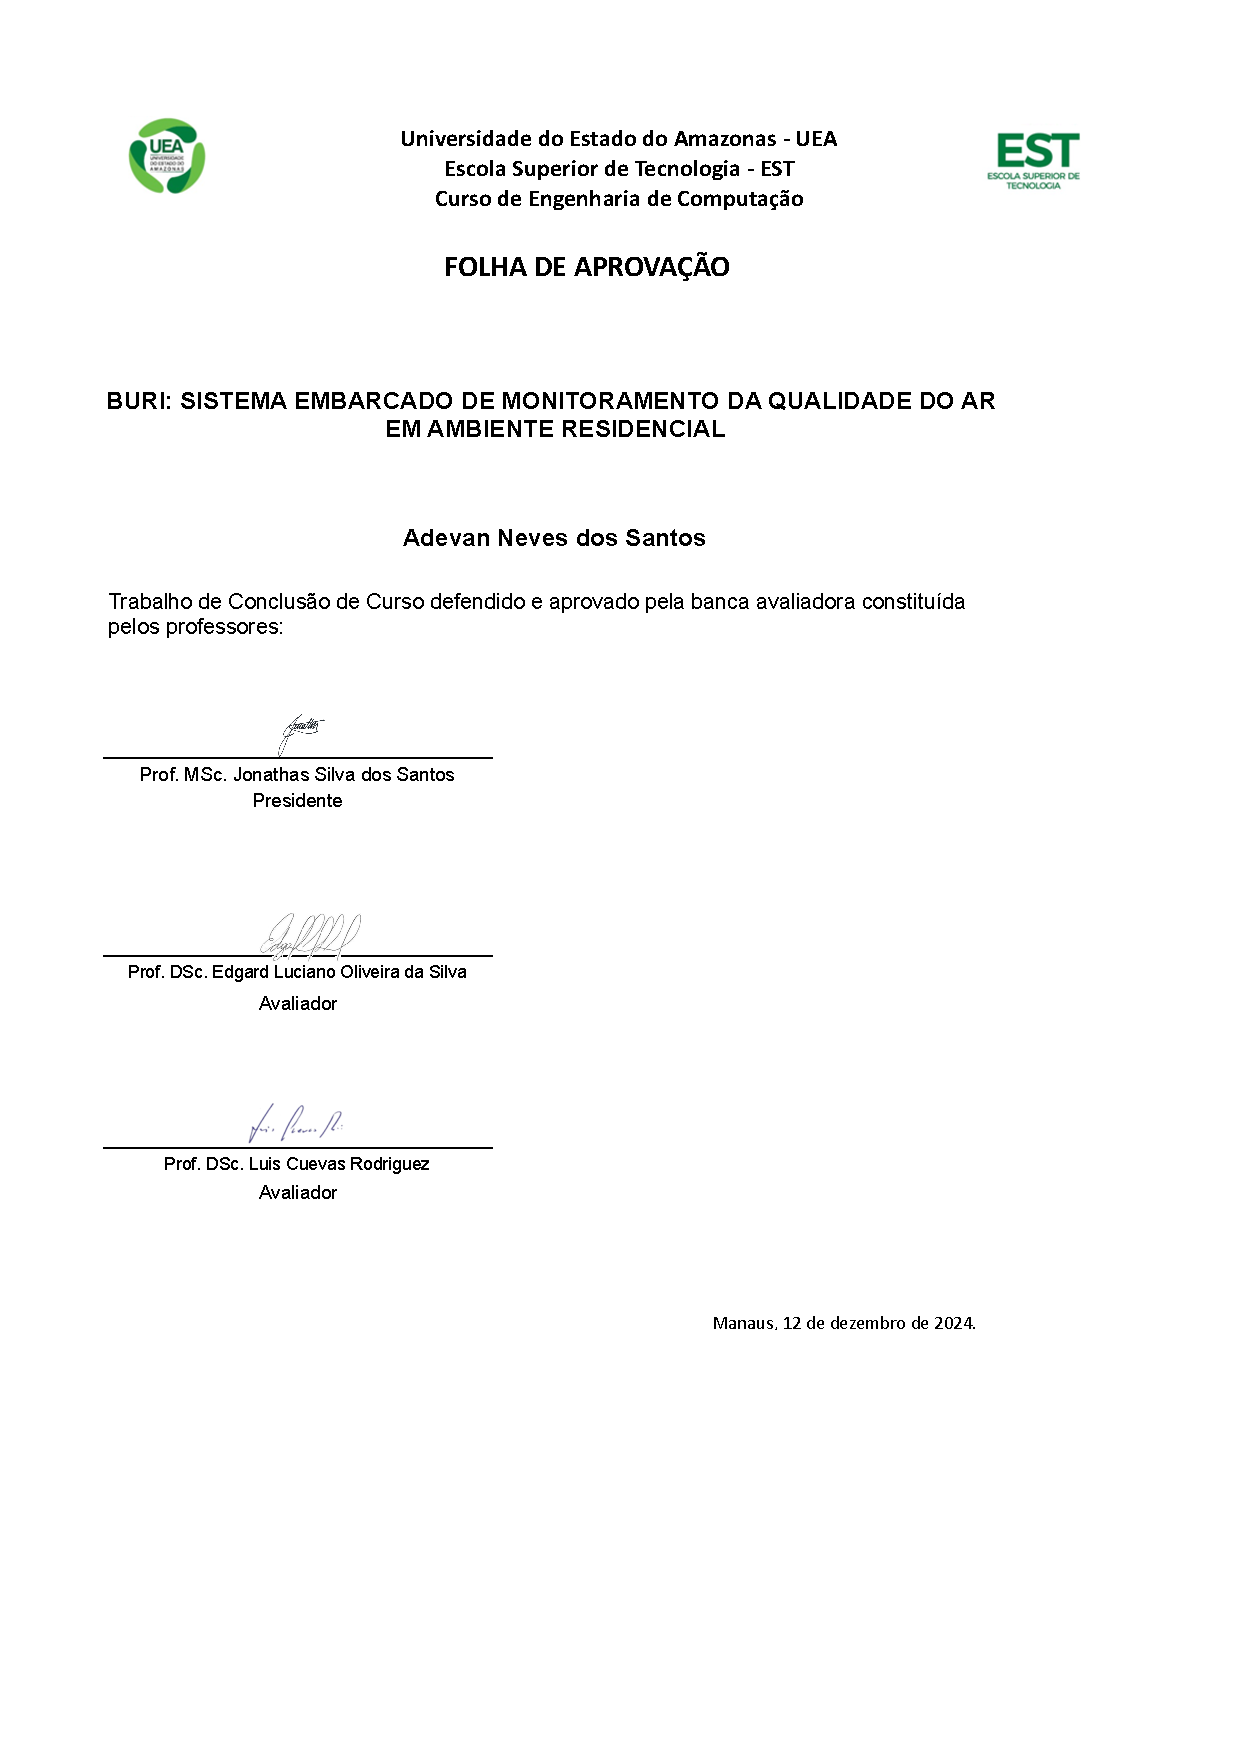
\includepdf[pages=-]{./source/assinaturas.pdf}
   \end{verbatim}
\end{enumerate}

\newpage
